\chapter{Memoria virtuale}

\section{Introduzione}
I metodi di gestione della Memoria Primaria (MP) cercano di mantenere in RAM il maggior numero possibile di processi per aumentare il livello di multiprogrammazione. Tuttavia, per una data quantità di RAM disponibile, il numero di processi che possono risiedere in MP dipende dalla loro dimensione.

\dfn{Memoria Virtuale (MV)}{
La \emph{Memoria Virtuale (MV)} è un insieme di tecniche che permette l'esecuzione di processi in cui codice e/o dati non sono completamente caricati in Memoria Primaria. La MV funziona poiché i programmi non necessitano di essere interamente presenti in MP per poter essere eseguiti. 
}

\ex{Esempi di utilizzo della Memoria Virtuale}{
- Il codice per la gestione delle condizioni di errore potrebbe non essere mai usato durante l’esecuzione di un programma.
- Array, liste e tabelle sono spesso dichiarate di dimensioni superiori a quanto effettivamente richiesto.
- Alcune opzioni di programma sono raramente utilizzate.
- Le librerie dinamiche vengono caricate in RAM solo se e quando effettivamente richieste.
}

L’idea alla base della Memoria Virtuale è la seguente:
\begin{itemize}
    \item Carichiamo in MP solo le parti di un programma che devono effettivamente essere eseguite e solo quando è necessario.
    \item Carichiamo in MP solo la porzione di strutture dati che sono utilizzate in una determinata fase di esecuzione.
\end{itemize}

\clm{Vantaggi della Memoria Virtuale}{}{
La Memoria Virtuale permette di eseguire programmi che superano la dimensione della MP. Formalmente:
\begin{itemize}
    \item È possibile eseguire un processo che utilizza uno spazio di indirizzamento logico superiore allo spazio fisico disponibile.
    \item È possibile avere in esecuzione contemporaneamente più processi che, sommati, occupano più spazio della MP disponibile.
    \item Ne consegue un aumento della multiprogrammazione e quindi del \emph{throughput} della CPU.
    \item I programmi possono iniziare l’esecuzione più velocemente, poiché non è necessario caricarli interamente in memoria primaria.
\end{itemize}
}

Naturalmente, vi sono anche degli \emph{inconvenienti} legati all'uso della Memoria Virtuale:
\begin{itemize}
    \item Si genera un aumento del traffico tra la RAM e l’hard disk.
    \item L'esecuzione di un singolo programma potrebbe richiedere più tempo rispetto a uno scenario senza MV.
    \item In situazioni particolari, le prestazioni complessive del sistema possono degradare drasticamente, fenomeno noto come \emph{thrashing}.
\end{itemize}

\section{Paginazione su richiesta (Demand Paging)}
L'idea di base della Memoria Virtuale è quella di \emph{portare una pagina in MP solo nel momento del primo indirizzamento di una locazione} (un dato, un'istruzione) appartenente alla pagina stessa.
Quando la CPU esegue un'istruzione che indirizza una locazione di RAM in una pagina diversa da quella contenente l'istruzione in esecuzione, e la pagina non è in MP, si dice che il processo ha generato un \emph{page fault}. In questo caso, il Sistema Operativo (SO) deve:
\begin{enumerate}
    \item sospendere il processo,
    \item portare in memoria la pagina mancante,
    \item una volta disponibile, riprendere l'esecuzione del processo dal punto in cui era stato interrotto.
\end{enumerate}
\subsection*{Passaggi per la gestione del page fault}
Più in dettaglio, quando manca la pagina riferita:
\begin{itemize}
    \item Il processo viene tolto dalla CPU e messo in uno stato di \emph{waiting for page}.
    \item Un modulo del SO detto \emph{pager} inizia il caricamento della pagina mancante dalla Memoria Secondaria (MS) in un frame libero della Memoria Primaria (MP).
    \item Nel frattempo, la CPU viene assegnata a un altro processo.
    \item Quando la pagina è caricata in MP, il processo corrispondente viene rimesso in coda di \emph{Ready}: riprenderà l'esecuzione dall'istruzione che aveva causato il problema quando sarà scelto dallo scheduler.
\end{itemize}
\nt{Vedere Code di Scheduling, nel diagramma di accodamento del capitolo 3, il caso wait for an interrpt lo possiamo anche associare al page fault. \ref{fig:ready_queue}}
\subsection*{Come viene rilevata l'assenza di una pagina in MP}
La CPU determina la presenza di una pagina in RAM attraverso un \emph{bit di validità} associato a ogni entry della Page Table (PT). Questo bit indica se la pagina associata è effettivamente in MP:
\begin{itemize}
    \item Se si tenta di accedere a una pagina non in MP, il suo bit di validità sarà impostato a 0, e viene generata una \emph{trap} detta \emph{page fault}, attivando il meccanismo descritto.
    \item Quando la pagina viene caricata in MP, il bit di validità viene impostato a 1 e la PT aggiornata; a questo punto, il processo può riprendere dall'istruzione che aveva causato il page fault.
\end{itemize}
\subsection*{Pure Demand Paging}
Un processo può persino iniziare senza alcuna delle sue pagine in MP. Al primo indirizzamento da parte del Program Counter (PC), che è inizializzato dal SO, si genera un \emph{page fault} perché il PC punta a una pagina non in MP del processo. Questo approccio è detto \emph{Pure Demand Paging}.

\nt{In alternativa, il SO può caricare in MP almeno la pagina contenente la prima istruzione da eseguire.}
\begin{figure}[h] \centering 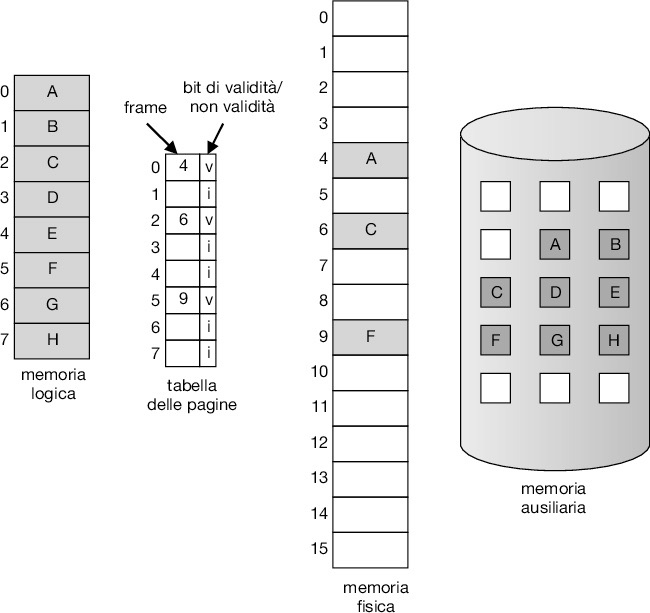
\includegraphics[width=0.25\linewidth]{images/table_of_pages_notAllInRam.png} \caption{table_of_pages_notAllInRam.png} \label{fig:10.4} \end{figure}
\begin{figure}[h] \centering 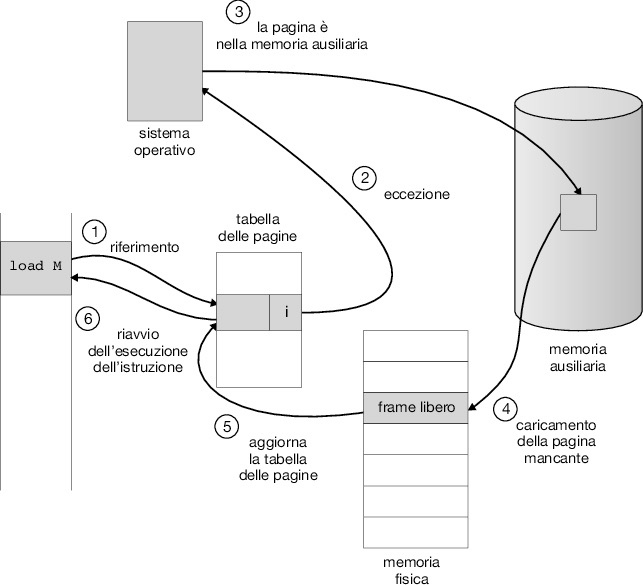
\includegraphics[width=0.25\linewidth]{images/page_fault_gestion.png} \caption{page_fault_gestion.png} \label{fig:10.5} \end{figure}

\section{Demand Paging}
\nt{
    Un processo può essere avviato senza che alcuna delle sue pagine sia inizialmente in Memoria Primaria (MP). Alla prima istruzione indirizzata dal Program Counter (PC), inizializzato dal Sistema Operativo (SO), si genera un \emph{page fault}, poiché il PC punta a un indirizzo di una pagina del processo non presente in MP. Questo schema è chiamato \emph{Pure Demand Paging}.
}

In alternativa, il SO può caricare preventivamente in MP almeno la pagina contenente la prima istruzione da eseguire.

\section*{Supporto Hardware per la Memoria Virtuale}

\nt{
    Per implementare la memoria virtuale è necessario un supporto hardware specifico:
    \begin{itemize}
        \item La tabella delle pagine deve includere un \emph{bit di validità} che l’hardware può testare per generare il \emph{page fault}.
        \item Le istruzioni devono essere ri-eseguibili in caso di \emph{page fault} oppure, alternativamente, l’hardware della CPU deve controllare la presenza in MP di tutti gli operandi prima di eseguire l'istruzione.
    \end{itemize}
}

\nt{
    Sebbene la paginazione possa essere aggiunta a qualsiasi sistema, la \emph{paginazione su richiesta} e, più in generale, la \emph{memoria virtuale}, richiedono un supporto hardware specifico.
}

\section*{Tempo di Accesso Effettivo}

Supponiamo di dover leggere un dato in MP:
\begin{itemize}
    \item \emph{ma} = tempo di accesso in MP se il dato è presente (es. 100-200 nanosecondi)
    \item \emph{p} = probabilità di un page fault
    \item \emph{eat} (effective access time) = 
    \[
    \text{eat} = [(1 - p) \times ma] + [p \times \text{tempo di gestione del page fault}]
    \]
\end{itemize}
